\smallframetitle

\section{From 29/07/24 to 02/08/24}
\insertsectionframe

\subsection{Methodology for Identifying True Neighboring Base Stations Based on Antenna Azimuths}
\insertsubsectionframe


\begin{frame}
    \frametitle{Improved Methodology}
    The goal is to identify true neighboring base stations by analyzing antenna azimuths.
    \begin{block}{Azimuth approach}
        True neighbors are stations within each others line of sight and within the coverage range of their directed antennas.
    \end{block}
    \begin{block}{Defining Coverage Angles}
        \begin{itemize}
            \item \textbf{Antenna beamwidth}
            \begin{itemize}
                \item Each antenna has a specified azimuth and coverage angle (beamwidth).
                \item Coverage angles are calculated based on azimuth direction and beamwidth, giving start and end angles.
            \end{itemize}
            \item \textbf{Steps to Define Coverage Angles:}
            \begin{itemize}
                \item For an antenna with azimuth \( A \) and beamwidth \( B \):
                \begin{itemize}
                    \item Coverage Start Angle = \( A - \frac{B}{2} \)
                    \item Coverage End Angle = \( A + \frac{B}{2} \)
                \end{itemize}
            \end{itemize}
        \end{itemize}
    \end{block}
\end{frame}

\begin{frame}{Verification Process}
    \begin{block}{Step-by-Step Validation}
        \textbf{Step 1: Calculate the Direction of the Connecting Line:}
        \begin{itemize}
            \item Determine the azimuth angle of the line connecting the two base stations.
        \end{itemize}
        \textbf{Step 2: Validate Antenna Direction for Both Base Stations:}
        \begin{itemize}
            \item Check if the connecting line’s direction falls within the coverage angles of its antennas.
        \end{itemize}
        \textbf{Step 3: Determine the Shorter Angle:}
        \begin{itemize}
            \item Calculate the angle between the azimuth of the antenna and the direction of the connecting line.
            \item Measure the smaller angle between the azimuth and the connecting line direction.
        \end{itemize}
        \textbf{Step 4: Check Bi-Directional Coverage:}
        \begin{itemize}
            \item Perform validation from both base stations’ perspectives.
            \item If conditions are met for both, consider them true neighbors.
        \end{itemize}
        \textbf{Step 5: Applying the Distance Criterion:}
    \end{block}
\end{frame}

\begin{frame}{Analysis of Results}
    \begin{columns}
        \begin{column}{0.5\textwidth}
            \begin{figure}
                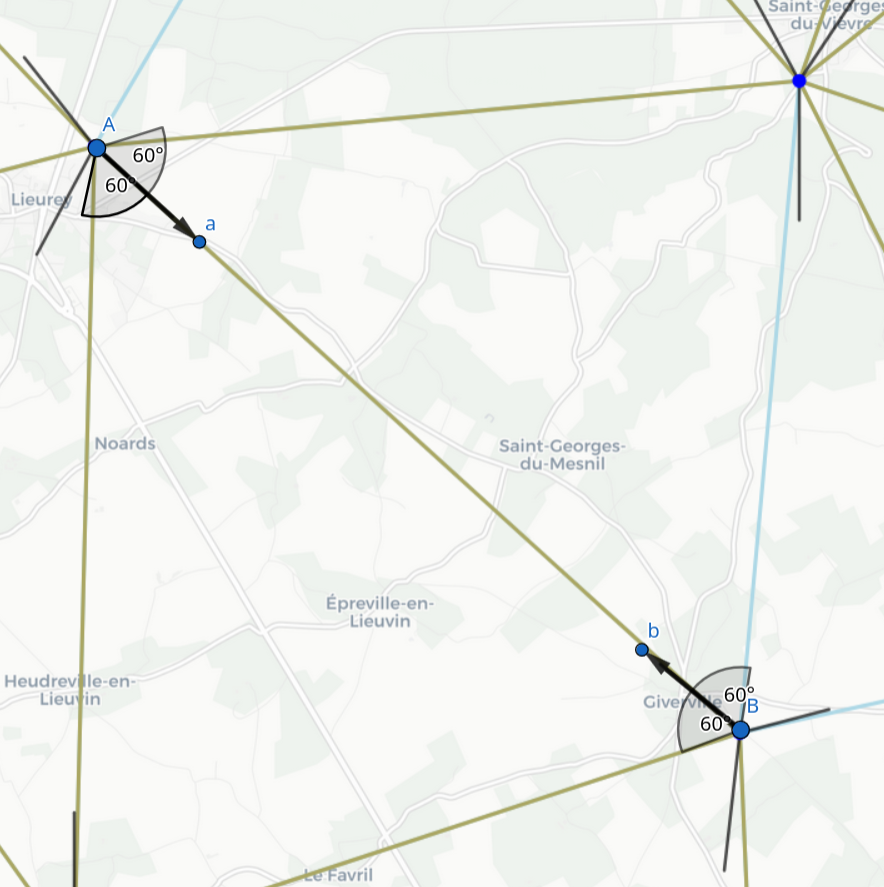
\includegraphics[height=0.3\paperwidth]{images/Altair/azimuth_expl.png}
                \caption{Visualization of the antenna coverage angle based methodology}
            \end{figure}
        \end{column}
        \begin{column}{0.5\textwidth}
            \begin{figure}
                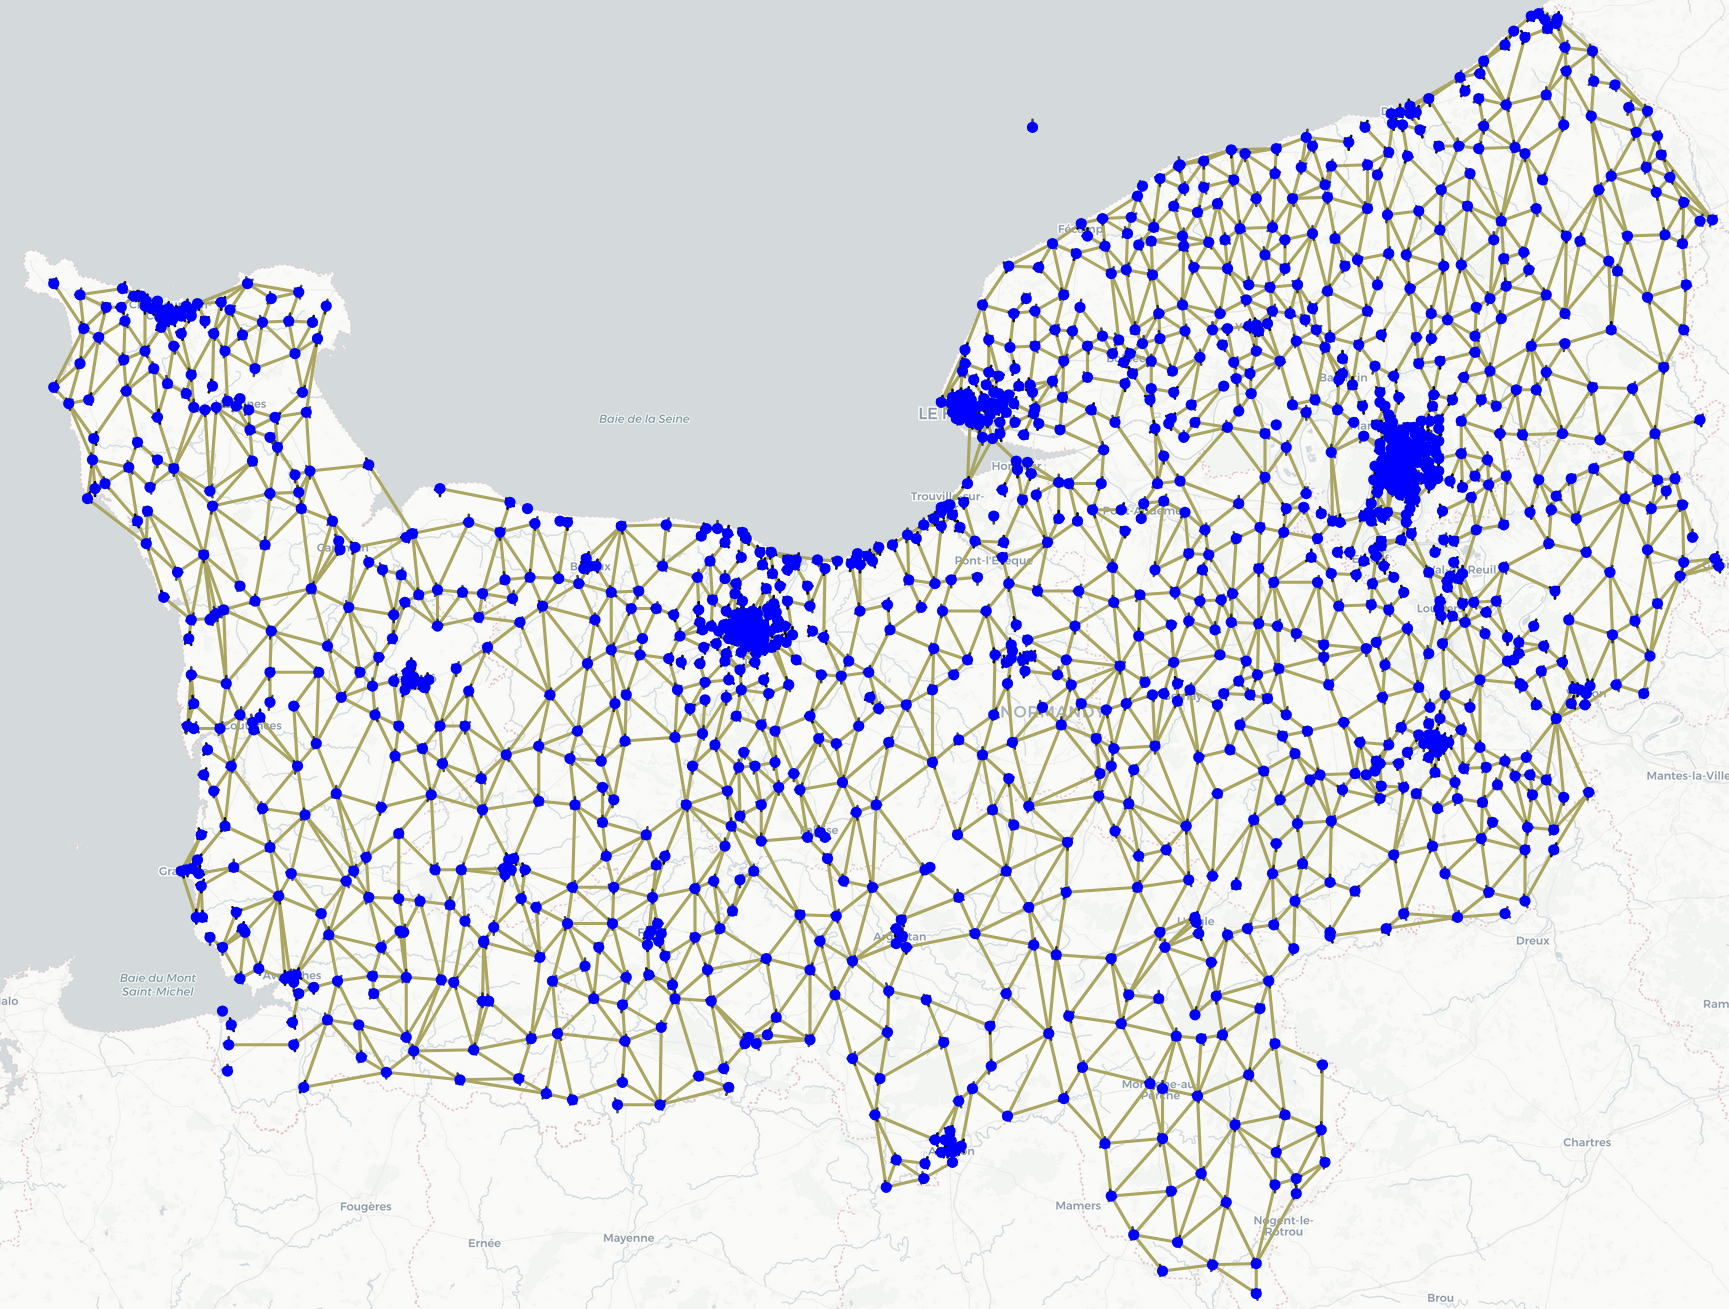
\includegraphics[height=0.6\paperheight]{images/Altair/azimuth_neigh_detect_normandy.png}
                \caption{Results on the map}
            \end{figure}
        \end{column}
    \end{columns}        
\end{frame}

\begin{frame}{Issue with Directional Antenna Coverage Methodology}
    \begin{columns}
        \begin{column}{0.5\textwidth}
            \begin{block}{Problem Explanation}
                \begin{itemize}
                    \item The current methodology focuses on identifying neighboring base stations based on the directional coverage of their antennas.
                    \item However, this approach can miss real neighboring stations that have overlapping coverage areas but whose antennas are not directly oriented towards each other.
                    \item As a result, some base stations that are effectively neighbors in terms of coverage might be excluded from the neighbor graph.
                    \item This limitation highlights the need for a more nuanced approach that considers not just the directional angles but also the actual coverage areas.
                \end{itemize}
            \end{block}
        \end{column}
        \begin{column}{0.5\textwidth}
            \begin{figure}
                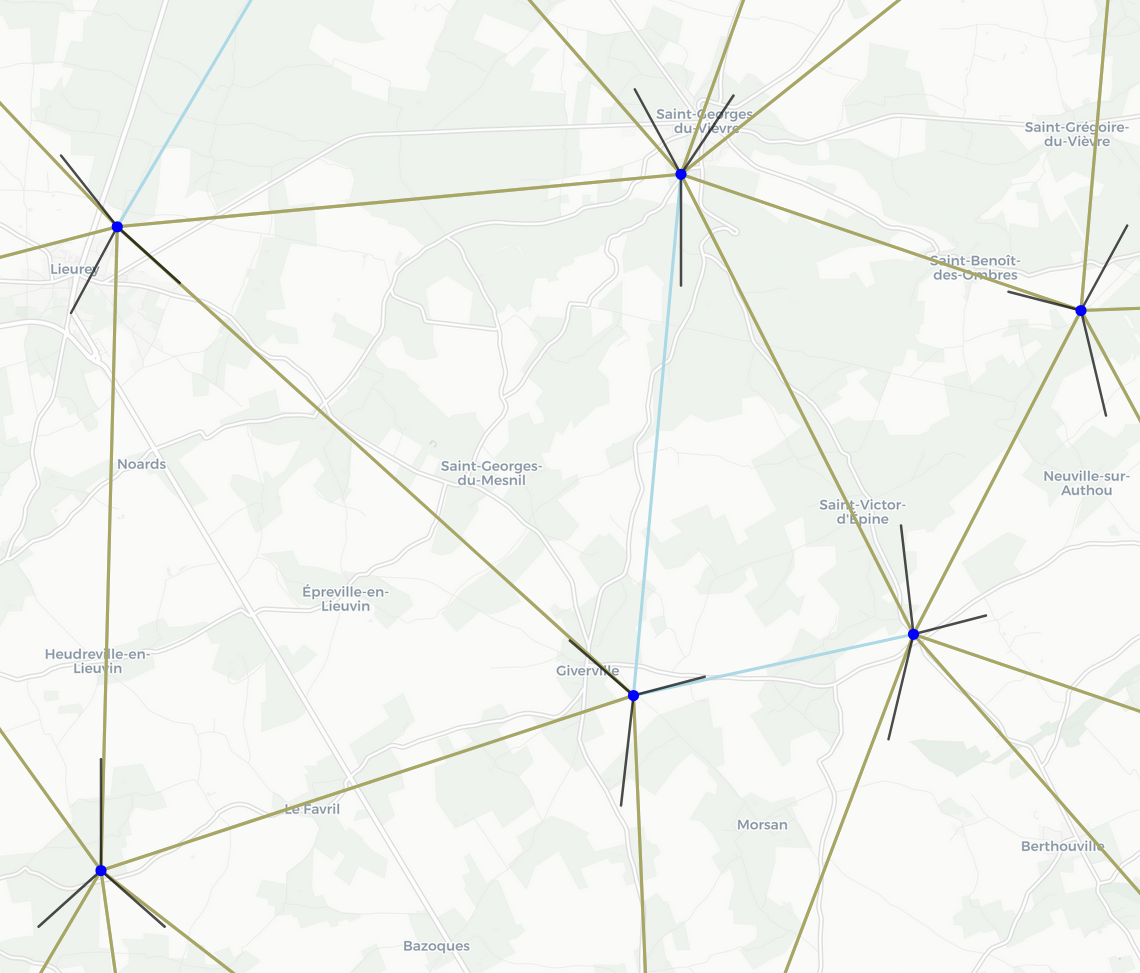
\includegraphics[width=0.7\textwidth]{images/Altair/problem_with_azimuth.png}  
                \caption{Coverage Overlap Issue}
            \end{figure}
        \end{column}
    \end{columns}
\end{frame}

\subsection{State of the art of different methods}
\insertsubsectionframe

\begin{frame}{Modification of criteria}
    \begin{block}{New angle values}
        For each category, we will apply a different angle criterion :
        \begin{itemize}
            \item $\gamma\in\left]0, 1\right]$: $\text{min\_angle}=5^\circ$;
            \item $\gamma\in\left]1, 2\right]$: $\text{min\_angle}=10^\circ$;
            \item $\gamma\in\left]2, 4\right]$: $\text{min\_angle}=15^\circ$;
            \item $\gamma\in\left]4, \infty\right[$: $\text{min\_angle}=20^\circ$.
        \end{itemize}
    \end{block}

    \begin{block}{New quadrant criterion}
        The idea is to use azimuths of each base station to make quadrants but as you will see results are really bad.
    \end{block}
\end{frame}

\begin{frame}{How to compare different methods (1/2)}
    For the comparison between the different methods we will need to put in place a way to compute dissimilarity between two methods.
    \begin{block}{Dissimiliarity computation}
        Let $\Delta$ be the value we are looking for. Let $\alpha$ the number of edges in method 1 not in method 2 and $\beta$ the number of edges in method 2 not in method 1. So, we have:
        $$
            \Delta = \alpha + \beta
        $$
    \end{block}
    And here is what we have when we compare to azimuth method :
    \begin{table}[!ht]
        \small
        \centering
        \begin{tabular}{lr}
            Delaunay: & $\alpha = 0, \beta = 1008, \Delta = 1008$\\
            Gabriel graph: & $\alpha = 684, \beta = 589, \Delta = 1273$\\
            7-NN: & $\alpha = 302, \beta = 3095, \Delta = 3397$\\
            15-NN: & $\alpha = 19, \beta = 9699, \Delta = 9718$\\
        \end{tabular}
        \caption{Dissimiliarity with unfiltered methods}
    \end{table}
\end{frame}

\begin{frame}{How to compare different methods (2/2)}
    \begin{table}[!ht]
        \tiny
        \centering
        \begin{columns}
            \begin{column}{0.5\paperwidth}
                \begin{tabular}{lr}
                    Delaunay and simple-criteria [adq]: & $\alpha = 919, \beta = 477, \Delta = 1396$\\
                    Delaunay and enhanced-criteria [adq]: & $\alpha = 873, \beta = 464, \Delta = 1337$\\
                    Delaunay and enhanced-criteria\_v2 [adq]: & $\alpha = 1751, \beta = 362, \Delta = 2113$\\
                    Gabriel graph and enhanced-criteria [adq]: & $\alpha = 1098, \beta = 433, \Delta = 1531$\\
                    7-NN and enhanced-criteria [adq]: & $\alpha = 1023, \beta = 524, \Delta = 1547$\\
                    15-NN and enhanced-criteria [adq]: & $\alpha = 899, \beta = 620, \Delta = 1519$\\
                    \hline
                    Delaunay and simple-criteria [aqd]: & $\alpha = 919, \beta = 477, \Delta = 1396$\\
                    Delaunay and enhanced-criteria [aqd]: & $\alpha = 873, \beta = 466, \Delta = 1339$\\
                    Delaunay and enhanced-criteria\_v2 [aqd]: & $\alpha = 1751, \beta = 362, \Delta = 2113$\\
                    Gabriel graph and enhanced-criteria [aqd]: & $\alpha = 1098, \beta = 435, \Delta = 1533$\\
                    7-NN and enhanced-criteria [aqd]: & $\alpha = 1021, \beta = 525, \Delta = 1546$\\
                    15-NN and enhanced-criteria [aqd]: & $\alpha = 893, \beta = 612, \Delta = 1505$\\
                    \hline
                    Delaunay and simple-criteria [daq]: & $\alpha = 919, \beta = 477, \Delta = 1396$\\
                    Delaunay and enhanced-criteria [daq]: & $\alpha = 873, \beta = 464, \Delta = 1337$\\
                    Delaunay and enhanced-criteria\_v2 [daq]: & $\alpha = 1751, \beta = 361, \Delta = 2112$\\
                    Gabriel graph and enhanced-criteria [daq]: & $\alpha = 1098, \beta = 433, \Delta = 1531$\\
                    7-NN and enhanced-criteria [daq]: & $\alpha = 1023, \beta = 524, \Delta = 1547$\\
                    15-NN and enhanced-criteria [daq]: & $\alpha = 898, \beta = 620, \Delta = 1518$\\
                \end{tabular}
            \end{column}
            \begin{column}{0.5\paperwidth}
                \begin{tabular}{lr}
                    Delaunay and simple-criteria [dqa]: & $\alpha = 930, \beta = 489, \Delta = 1419$\\
                    Delaunay and enhanced-criteria [dqa]: & $\alpha = 885, \beta = 470, \Delta = 1355$\\
                    Delaunay and enhanced-criteria\_v2 [dqa]: & $\alpha = 1755, \beta = 393, \Delta = 2148$\\
                    Gabriel graph and enhanced-criteria [dqa]: & $\alpha = 1098, \beta = 431, \Delta = 1529$\\
                    7-NN and enhanced-criteria [dqa]: & $\alpha = 1035, \beta = 540, \Delta = 1575$\\
                    15-NN and enhanced-criteria [dqa]: & $\alpha = 938, \beta = 645, \Delta = 1583$\\
                    \hline
                    Delaunay and simple-criteria [qad]: & $\alpha = 930, \beta = 489, \Delta = 1419$\\
                    Delaunay and enhanced-criteria [qad]: & $\alpha = 883, \beta = 470, \Delta = 1353$\\
                    Delaunay and enhanced-criteria\_v2 [qad]: & $\alpha = 1755, \beta = 393, \Delta = 2148$\\
                    Gabriel graph and enhanced-criteria [qad]: & $\alpha = 1098, \beta = 433, \Delta = 1531$\\
                    7-NN and enhanced-criteria [qad]: & $\alpha = 1032, \beta = 540, \Delta = 1572$\\
                    15-NN and enhanced-criteria [qad]: & $\alpha = 935, \beta = 638, \Delta = 1573$\\
                    \hline
                    Delaunay and simple-criteria [qda]: & $\alpha = 930, \beta = 489, \Delta = 1419$\\
                    Delaunay and enhanced-criteria [qda]: & $\alpha = 883, \beta = 470, \Delta = 1353$\\
                    Delaunay and enhanced-criteria\_v2 [qda]: & $\alpha = 1755, \beta = 393, \Delta = 2148$\\
                    Gabriel graph and enhanced-criteria [qda]: & $\alpha = 1098, \beta = 433, \Delta = 1531$\\
                    7-NN and enhanced-criteria [qda]: & $\alpha = 1032, \beta = 540, \Delta = 1572$\\
                    15-NN and enhanced-criteria [qda]: & $\alpha = 935, \beta = 638, \Delta = 1573$\\
                \end{tabular}
            \end{column}
        \end{columns}
        \caption{Dissimiliarity with filtered methods}
    \end{table}
\end{frame}

\subsection{Mean distances in departments}
\insertsubsectionframe

\begin{frame}{How all is constructed}
    The \texttt{Population}, \texttt{Superficie} and \texttt{Densite} data is from here : \url{https://france.ousuisje.com/departements/classement/superficie.php}.

    \begin{block}{Mean distance calculation}
        Let $M$ be the value we are looking for. Let $S$ be the set of one department's base stations. Let $N_j$ be the set of distances to $j$'s nearest neighbours, we will keep $10$ of them.
        \[
            M = \frac{\sum_{j\in S}\frac{\sum_{i\in N_j, i\leqslant 10}{(N_j)_i}}{\mathrm{\mathop{size}}(N_j)}}{\mathrm{\mathop{size}}(S)}
        \]
        So $M$ is the value called \texttt{total}.

        For \texttt{countryside}, it's the same calculation but only on counstryside's base stations. For \texttt{city}, we have an additional criterion to get rid of bad values:
        we only keep, in the $10$ nearest neighbours, the one that are less than $\unit[6]{km}$ distant.

        By the way, all those values are in $\unit{km}$.
    \end{block}

    We can also normalize these values with this formula: $M_{norm}=\frac{M-\min(Ms)}{\max(Ms)-\min(Ms)}$, where $Ms$ is the set of $M$ values for all departments.
\end{frame}

\begin{frame}{Results}
    \begin{table}[!ht]
        \tiny
            \centering
            \begin{tabular}{l|lllllllll}
                \textbf{nom\_dep} & \textbf{Population} & \textbf{Superficie} & \textbf{Densite} & \textbf{city} & \textbf{countryside} & \textbf{total} & \textbf{normalized\_city} & \textbf{normalized\_countryside} & \textbf{normalized\_total} \\ \hline
                \textbf{Paris} & 2166200 & 105 & 20433 & 0.21439 & -1 & 0.21439 & 0 & 0 & 0 \\ 
                \textbf{Hauts-de-Seine} & 1517000 & 176 & 8619 & 0.4315 & -1 & 0.4315 & 0.07834 & 0 & 0.05889 \\ 
                
                \textbf{Rhône} & 1667500 & 3249 & 513 & 1.04954 & 8.52619 & 1.08092 & 0.30134 & 0.79741 & 0.23503 \\ 
                
                \textbf{Hérault} & 992500 & 6224 & 159 & 1.66912 & 7.83726 & 1.81089 & 0.52491 & 0.73974 & 0.43303 \\ 
                \textbf{Loire-Atlantique} & 1209000 & 6815 & 177 & 1.75516 & 8.15056 & 1.99532 & 0.55595 & 0.76597 & 0.48305 \\ 
                \textbf{Bas-Rhin} & 1063000 & 4755 & 224 & 1.78152 & 7.51702 & 1.7444 & 0.56546 & 0.71294 & 0.41499 \\ 
                \textbf{Haute-Savoie} & 631679 & 4388 & 144 & 1.81713 & 8.8195 & 1.78003 & 0.57831 & 0.82196 & 0.42466 \\ 
                
                \textbf{Gironde} & 1376000 & 10000 & 138 & 1.89034 & 8.44384 & 2.09651 & 0.60473 & 0.79052 & 0.5105 \\ 
                \textrm{\textbf{Seine-Maritime}} & 1245000 & 6278 & 198 & 1.89128 & 7.1899 & 1.95555 & 0.60507 & 0.68555 & 0.47226 \\ 
                \textbf{Pas-de-Calais} & 1456000 & 6671 & 218 & 1.92476 & 7.49829 & 1.96731 & 0.61715 & 0.71137 & 0.47545 \\ 
                
                \textbf{Ille-et-Vilaine} & 930000 & 6775 & 133 & 2.08199 & 7.58191 & 2.2183 & 0.67388 & 0.71837 & 0.54353 \\ 
                \textrm{\textbf{Calvados}} & 664000 & 5548 & 120 & 2.14504 & 8.43249 & 2.44803 & 0.69663 & 0.78957 & 0.60584 \\ 
                \textbf{Haute-Corse} & 148000 & 4666 & 30 & 2.15674 & 9.06187 & 2.75204 & 0.70085 & 0.84225 & 0.6883 \\ 
                
                \textbf{Indre-et-Loire} & 571500 & 6127 & 93 & 2.23539 & 8.35991 & 2.43487 & 0.72923 & 0.78349 & 0.60227 \\ 
                \textbf{Hautes-Pyrénées} & 222368 & 4464 & 50 & 2.3107 & 9.45288 & 2.80779 & 0.75641 & 0.87498 & 0.70342 \\ 
                \textbf{Finistère} & 852418 & 6733 & 127 & 2.32578 & 8.18865 & 2.52294 & 0.76185 & 0.76916 & 0.62616 \\ 
                
                \textrm{\textbf{Orne}} & 292337 & 6103 & 48 & 2.41672 & 10.6345 & 3.74098 & 0.79466 & 0.97389 & 0.95653 \\ 
                \textbf{Drôme} & 457651 & 6530 & 67 & 2.42289 & 7.99711 & 2.51054 & 0.79689 & 0.75312 & 0.62279 \\ 
                \textbf{Ariège} & 137205 & 4890 & 28 & 2.44526 & 9.0807 & 2.83295 & 0.80496 & 0.84383 & 0.71024 \\ 
                
                \textbf{Cantal} & 150772 & 5726 & 26 & 2.55952 & 9.05477 & 2.95966 & 0.84619 & 0.84166 & 0.74461 \\ 
                \textbf{Jura} & 250857 & 4999 & 50 & 2.56287 & 8.79631 & 2.74338 & 0.8474 & 0.82002 & 0.68595 \\ 
                
                \textrm{\textbf{Manche}} & 489500 & 5938 & 82 & 2.74607 & 8.70393 & 3.14209 & 0.9135 & 0.81229 & 0.79409 \\ 
                \textbf{Creuse} & 124470 & 5565 & 22 & 2.76393 & 9.53859 & 3.53196 & 0.91994 & 0.88216 & 0.89984 \\ 
                
                \textrm{\textbf{Eure}} & 541054 & 6040 & 90 & 2.8698 & 7.90577 & 2.93429 & 0.95814 & 0.74548 & 0.73773 \\ 
                \textbf{Haute-Loire} & 209113 & 4977 & 42 & 2.88781 & 7.69017 & 2.85588 & 0.96464 & 0.72743 & 0.71646 \\ 
                \textbf{Aveyron} & 271200 & 8735 & 31 & 2.91637 & 8.62305 & 3.11151 & 0.97495 & 0.80552 & 0.7858 \\ 
                
                \textbf{Dordogne} & 401500 & 9060 & 43 & 2.9858 & 8.06246 & 3.04884 & 1 & 0.75859 & 0.7688 \\ 
            \end{tabular}
            \caption{Mean distances (extract), \emph{sorted by \texttt{city}} [in roman \textrm{Normandy}]}
        \end{table}
\end{frame}